% ===========================================================================
\section{Extension: models beyond $\Lambda$CDM}\label{sec:models}
% ===========================================================================

The code has a library of eleven dark-energy and modified-gravity models beyond $\Lambda$CDM (twelve
configurations, since DGP has two branches). This section describes how
a model is organized in the code, the equations of each model, and how it is validated. All models are selected by
name in the parameter file (\texttt{model = ...}), and the model parameters are set there too.

\subsection{Species and gravity}

A model is a list of \emph{species} and a theory of \emph{gravity}. A species provides its background density and
pressure, $\rho(x)$ and $p(x)$, and the first two derivatives of $\rho$. If it clusters, it also has a perturbation
block: its variables, initial conditions and equations. The block is coupled to the metric only through four
moments: $\delta\rho$, $\delta p$, the momentum $(\rho+p)\theta/k$ and the shear $(\rho+p)\sigma$. It receives
$\Phi$, $\Psi$ and $\Phi'$ in return. Interacting components, such as dark matter coupled to dark energy, are a
single block that holds the variables of both. The gravity gives $E^2=H^2/H_0^2$ from the species. It also owns its
own perturbation variables: $\Phi$ in GR, and $\Phi$ plus two scalar-field variables in the scalar--tensor theories.
From these and the summed moments it computes $\Phi$, $\Psi$ and $\Phi'$. Photons and baryons, with Thomson scattering,
tight coupling and the line-of-sight sources, are the fixed core of the perturbation module. All models use the same
conventions as Sec.~\ref{sec:m3}: conformal Newtonian gauge, $x=\ln a$ and our sign of $\Phi$. Below, the spatial
potential is written with the Planck sign, $\Phi_P=-\Phi$.

Every model is tested in its GR/$\Lambda$CDM limit. Where possible we also check the Einstein constraint equations
that the code does not integrate. Some models evolve $\Phi$ with the energy constraint but not the momentum
constraint; in an interacting model the momentum constraint holds only if the exchanged energy and momentum cancel
between the species. We test the growth of structure on sub-horizon scales against independent solutions of the
quasi-static growth equation, and compare with CLASS, hi\_class and CLASS\_EDE where possible. Table~\ref{tab:models}
summarizes the models, and Figs.~\ref{fig:models_de} and \ref{fig:models_mg} show their effects for the parameters
of the table. All other parameters are those of the fiducial model; $\Om_\Lambda$, or the density of the dark-energy
field, is set by closure. The runs use RECFAST and include lensing.

\subsection{Dark energy and dark-sector interactions}

\paragraph*{Quintessence (\texttt{quintessence}).} A minimally coupled scalar field with potential
$V=3H_0^2M_{\rm pl}^2V_0e^{-\lambda\phi}$ (the field $\phi$ is in units of $M_{\rm pl}$). It starts at rest in the
radiation era, where Hubble friction freezes it, and $V_0$ is found by shooting so that the field closes the
universe. With $\phi_x=d\phi/dx$, the background equations are
\begin{equation}
E^2=\frac{\rho_o+v}{1-\phi_x^2/6},\quad
\phi_{xx}=-\Big(3+\frac{d\ln E}{dx}\Big)\phi_x-\frac{3v_\phi}{E^2},
\end{equation}
where $v=V/(3H_0^2M_{\rm pl}^2)$ and $\rho_o$ is the density of the other species. The field perturbation $\delta\phi$
obeys the Klein--Gordon equation of Mukhanov. We evolve $\delta\phi$ and $w=\delta\phi_x-\phi_x\Psi$; the
combination $w$ removes $\Psi'$ from the equation. \emph{Validation:} the background agrees with an independent
integration in cosmic time, and the Poisson and momentum constraints hold to $10^{-7}$ with the field's density and
momentum.

\paragraph*{Coupled quintessence (\texttt{coupled\_quintessence}).} The dark matter particle mass depends on the
field, $m\propto e^{-\beta\phi}$~\cite{Wetterich1995,Amendola2000}. This gives
\begin{equation}
\rho_c'=-(3+\beta\phi_x)\rho_c,\quad
\phi_{xx}=\dots-\frac{3v_\phi}{E^2}+\frac{3\beta\rho_c}{E^2}.
\end{equation}
The dark matter feels a fifth force, which makes its effective gravitational constant $G(1+2\beta^2)$ on small
scales. It also feels a drag term $\propto\beta\phi_xv_c$. \emph{Validation:} an independent integration in cosmic
time with the coupling; the constraint equations, which hold only if the exchange cancels; and the dark matter
growth with fifth force and drag.

\paragraph*{Dark scattering (\texttt{dark\_scattering}).} Elastic scattering between dark matter and a dark-energy
fluid with constant $w$ and sound speed $\hat c_s^2$~\cite{Simpson2010}. The cross section per unit mass is
$\xi=\sigma_D/m_c$. Only momentum is exchanged, with rates $\Gamma_{\rm DE}=ac\xi\rho_c$ and
$\Gamma_c=(1+w)(\rho_{\rm DE}/\rho_c)\Gamma_{\rm DE}$. At early times $\Gamma_{\rm DE}\gg\Hp$, and the
dark-energy velocity is locked to that of the dark matter. \emph{Validation:} the constraints with momentum exchange;
the drag in the growth against two-fluid growth equations ($5\times10^{-4}$); and, for $\xi=0$, the wCDM/$\Lambda$CDM
ratios against CLASS's fluid dark energy (P(k) to $5\times10^{-5}$, TT to $2\times10^{-4}$ for $\ell\le800$).

\paragraph*{Early dark energy (\texttt{ede}).} An axion-like field with
$V=m^2f^2(1-\cos\phi/f)^n$~\cite{Poulin2019,Smith2020}, plus a cosmological constant. The field is frozen at
$\theta_i=\phi_i/f$ until $H\sim m$. It then oscillates, and its energy dilutes as $a^{-6n/(n+1)}$. The model is
specified as in CLASS\_EDE~\cite{Hill2020}, by the maximum fraction $f_{\rm EDE}$ of the total density, its
redshift $z_c$, $\theta_i$ and $n$. A Newton iteration on $(\ln m^2f^2,\ln f)$ finds the potential, and $\Om_\Lambda$
follows from closure. For $n\le2$ the oscillating field does not dilute faster than radiation, so its fraction does
not peak and $(f_{\rm EDE},z_c)$ do not define the model; the code rejects these cases. The background and the
perturbations are integrated through all oscillations, with the Klein--Gordon equations of quintessence. Both
models share one scalar-field class. A run takes about 90\,s instead of 65\,s for $\Lambda$CDM. \emph{Validation:}
the shooting reproduces $f_{\rm EDE}$ and $z_c$ to $10^{-10}$, and the oscillation-averaged dilution is
$a^{-4.50}$ for $n=3$. The constraints hold to $5\times10^{-6}$, and $f_{\rm EDE}\to0$ is $\Lambda$CDM. Compared
with CLASS\_EDE, the decay constant $f$ agrees to $10^{-3}$. The ratios to $\Lambda$CDM agree to $3\times10^{-5}$ in
$P(k)$ for $k\le0.05\hMpc$ ($7\times10^{-4}$ at $0.1\hMpc$) and to $10^{-3}$ in TT.

\paragraph*{Interacting dark energy (\texttt{ide}).} A dark-energy fluid with constant $w$ that exchanges energy
with the dark matter at the rate $Q=\xi H\rho_{\rm DE}$~\cite{Valiviita2008,Gavela2009}. The energy is transferred
along the dark-matter velocity, so the dark matter feels no drag:
\begin{equation}
\rho_{\rm DE}\propto a^{-3(1+w)-\xi},\quad
\rho_c=\frac{1}{a^3}\Big[\Om_c+\xi\Om_{\rm DE}\frac{1-a^{-(3w+\xi)}}{3w+\xi}\Big].
\end{equation}
In the perturbations, $H$ in $Q$ is replaced by the local expansion rate of the dark matter, $\Theta_c/3$. The
dark-energy pressure is transformed to the fluid rest frame with $\rho_{\rm DE}'$ including the transfer.
Momentum conservation then gives
$\theta_{\rm DE}'=\dots+\xi\Hp[\theta_{\rm DE}-\theta_c/(1+w)]$. The early-time instability of these
models~\cite{Valiviita2008} is avoided if the ``doom factor'' $d=\xi/[3(1+w)]$ is negative; the code rejects
$d>0$ and models with $\rho_c<0$ before today. \emph{Validation:} $\rho_c$ against an independent integration
($10^{-14}$); the constraints with energy exchange ($2\times10^{-6}$); and $\xi=0$ against the separate wCDM
implementation of dark scattering (identical). With $\xi=-0.1$ the dark matter loses energy uniformly, so
$\delta_c$ grows faster: $P(k)$ is 1.254 times that of $\Lambda$CDM at $k=0.1\hMpc$.

\subsection{Modified gravity}

\paragraph*{$\mu$--$\Sigma$ (\texttt{musigma}).} The Planck/DES
parameterization~\cite{Planck2018MG,DES2019MG}. It modifies the Poisson equations for the comoving density
$\rho\Delta$ by
\begin{equation}
k^2\Psi=-4\pi Ga^2\mu\,\rho\Delta,\quad k^2(\Phi_P+\Psi)=-8\pi Ga^2\Sigma\,\rho\Delta,
\end{equation}
with $\mu=1+\mu_0\Om_{\rm DE}(a)/\Om_{\rm DE,0}$ and similarly for $\Sigma$. On super-horizon scales,
$\rho\Delta\sim(k/\Hp)^2\delta\rho$, so computing the potentials from $\rho\Delta$ directly would lose all precision
there. We therefore evolve the GR potential of $\rho\Delta$ with an equation derived from energy--momentum
conservation. This equation reduces exactly to GR for $\mu=\Sigma=1$. \emph{Validation:} the potentials against the
algebraic relations, and the growth against an independent solution of the growth equation with $\mu(a)$
($<10^{-4}$).

\paragraph*{DGP (\texttt{dgp}).} The braneworld model~\cite{Dvali2000}. Its background is
$E=\epsilon\sqrt{\Om_{rc}}+\sqrt{\Om_{rc}+\rho/\rho_{c0}}$, on the normal branch ($\epsilon=-1$, with $\Lambda$) or
the self-accelerating branch ($\epsilon=+1$). Optionally the expansion is that of $\Lambda$CDM, as in N-body work.
The perturbations are quasi-static, with $\mu=1+1/(3\beta)$,
$\beta=1-2\epsilon(Hr_c/c)(1+\dot H/3H^2)$, and $\Sigma=1$~\cite{Koyama2006}. They use the $\mu$--$\Sigma$
equations. \emph{Validation:} as for $\mu$--$\Sigma$, with $\mu(a)$ from the background.

\paragraph*{Jordan--Brans--Dicke (\texttt{jbd}).} The scalar field $\phi$ multiplies $R$, with coupling $\omega$,
plus a cosmological constant~\cite{BransDicke1961}. $\phi_0$ is fixed so that the Newtonian constant measured
today is $G$, and $\Om_\Lambda$ follows from $E(0)=1$; both are found by iteration. The perturbations are evolved in
full ($\Phi$, $\delta\phi$, $\delta\phi'$). We derived them symbolically. \emph{Validation:} the background
equations; the matter-era solution $\phi\propto a^{1/(1+\omega)}$; the momentum constraint ($5\times10^{-8}$);
and the growth with $G_{\rm eff}=G\phi_0/\phi$.

\paragraph*{Hu--Sawicky $f(R)$ (\texttt{fr}).} Ref.~\cite{HuSawicki2007} with $f_R=-|f_{R0}|(R_0/R)^{n+1}$. The
expansion is that of $\Lambda$CDM to $\mathcal O(f_{R0})$. The perturbations are quasi-static, with the
scale-dependent
\begin{align}
\mu(k,a)&=\frac{1+4Q}{(1+3Q)(1+f_R)},\quad \Sigma=\frac{1}{1+f_R},\nonumber\\
Q&=\frac{k^2}{a^2}\frac{f_{RR}}{1+f_R}=\frac{k^2\lambda_C^2}{3a^2}.
\end{align}
Below the Compton wavelength of the scalaron, gravity is enhanced by 4/3. \emph{Validation:} $f_R(a)$, the Compton
wavelength and the limits of $\mu$; the potentials at every $k$; and the scale-dependent growth at each $k$
($2\times10^{-4}$).

\paragraph*{Cubic Galileon (\texttt{cubic\_galileon}).} The Lagrangian is $c_2X-g_3X\Box\phi$ on its tracker
solution~\cite{Deffayet2009,Barreira2013}, with $E^2=[\rho+\sqrt{\rho^2+4\Om_\phi}]/2$ and no free parameter beyond
those of $\Lambda$CDM ($w_0\approx-1.19$). The braided scalar perturbations are evolved in full. We derived them
covariantly and checked them with the identity $\nabla^\mu T_{\mu\nu}=(\nabla\cdot J)\phi_\nu$. \emph{Validation:}
the tracker relations ($E^4-\rho E^2=\Om_\phi$, $w=-2/(1+\Om_\phi)$); the momentum constraint with all braiding
terms ($3\times10^{-8}$); and the sub-horizon growth against the quasi-static $G_{\rm eff}$ ($7\times10^{-5}$). The
model is ruled out by the ISW--galaxy cross-correlation. Here it shows the strongest effects: $C_\ell^{\phi\phi}$ is
1.177 times the $\Lambda$CDM value at $\ell=100$.

\paragraph*{Horndeski in the $\alpha$ basis (\texttt{horndeski}).} Following Bellini and Sawicki~\cite{Bellini2014}
and hi\_class~\cite{Zumalacarregui2017}, the linear theory is described by the kineticity $\alpha_K$, the braiding
$\alpha_B$, the running of the Planck mass $\alpha_M=d\ln M_*^2/d\ln a$, and the background. We set $\alpha_T=0$,
as required by GW170817. We derived the Newtonian-gauge equations for $L=F(\phi)R/2+G_2(\phi,X)-G_3(\phi,X)\Box\phi$,
which realizes any $\alpha_K,\alpha_B,\alpha_M$. We then eliminated the functions $G_i$ using the definitions of
the $\alpha$'s, their time derivatives and the background equations, and reduced the system to first order in
$v=-\delta\phi/\phi'$ and $u=v'+\Psi$. The no-ghost and gradient-stability conditions,
\begin{align}
D&=\alpha_K+\tfrac32\alpha_B^2>0,\nonumber\\
Dc_s^2&=(2-\alpha_B)\Big[\frac{\alpha_B}{2}+\alpha_M-\frac{\dot H}{H^2}\Big]\nonumber\\
&\quad-\frac{\rho_m+p_m}{H^2M_*^2}+\frac{\dot\alpha_B}{H}>0,
\end{align}
are checked before a run. The expansion is $\Lambda$CDM or $w_0w_a$. The $\alpha$'s use the hi\_class
parameterizations $\alpha_X=c_X\Om_{\rm DE}(a)$, $c_Xa$ or constant. All terms of the scalar equation are
proportional to an $\alpha$ or to the dark-energy momentum, so nothing cancels catastrophically at early times when
$D\to0$. \emph{Validation:} the momentum constraint ($3\times10^{-8}$). Three theories rebuilt from their $\alpha$'s
reproduce the dedicated implementations: the cubic Galileon ($\alpha_K=6\Om_{\rm DE}$, $\alpha_B=2\Om_{\rm DE}$, to
$5\times10^{-9}$), quintessence ($\alpha_K=3(\rho+p)_\phi/H^2$, $2\times10^{-11}$), and Brans--Dicke on its own
expansion ($M_*^2=\phi$, $\alpha_M=-\alpha_B$, $\alpha_K=\omega\alpha_M^2$, $9\times10^{-9}$). Against hi\_class
the ratios to $\Lambda$CDM agree to $10^{-4}$ in $P(k)$ and $8\times10^{-4}$ in TT.

\begin{table*}
\caption{The models beyond $\Lambda$CDM, the parameters used in Figs.~\ref{fig:models_de}--\ref{fig:models_mg},
the treatment of the perturbations, and $\sigma_8$ and $P(k=0.1\hMpc)$ relative to $\Lambda$CDM (same primordial
spectrum, $\Om_{b}$, $\Om_{c}$ and $h$).}
\label{tab:models}
\begin{ruledtabular}
\begin{tabular}{llllcc}
Model & Parameters & Perturbations & Main validation & $\sigma_8/\sigma_8^{\Lambda\rm CDM}$ & $P/P^{\Lambda\rm CDM}$\\
\hline
quintessence & $\lambda=1$ & full field & constraints, bg. & 0.978 & 0.956\\
coupled quint. & $\lambda=0.5$, $\beta=0.05$ & full field + CDM & constraints, growth & 1.037 & 1.071\\
dark scattering & $w=-0.9$, $\xi=10$\,b/GeV & fluid + CDM & CLASS ($\xi=0$), drag & 0.962 & 0.925\\
EDE & $f_{\rm EDE}=0.12$, $z_c=3630$, $\theta_i=2.83$ & full field & CLASS\_EDE & 0.945 & 0.899\\
IDE & $\xi=-0.1$, $w=-0.95$ & fluid + CDM & constraints, wCDM limit & 1.124 & 1.254\\
$\mu$--$\Sigma$ & $\mu_0=0.3$, $\Sigma_0=0.1$ & $\mu$--$\Sigma$ & growth equation & 1.038 & 1.077\\
nDGP & $H_0r_c/c=1$, $\Lambda$CDM bg. & quasi-static & growth equation & 1.070 & 1.145\\
sDGP & $\Om_\Lambda=0$ & quasi-static & growth equation & 0.809 & 0.654\\
Brans--Dicke & $\omega=100$ & full field & constraints, $G_{\rm eff}$ & 1.043 & 1.093\\
$f(R)$ & $|f_{R0}|=10^{-5}$, $n=1$ & quasi-static $\mu(k,a)$ & scale-dep.\ growth & 1.073 & 1.066\\
cubic Galileon & --- & full field (braiding) & constraints, $G_{\rm eff}$ & 1.097 & 1.203\\
Horndeski & $c_K=1$, $c_B=0.6$, $c_M=0.3$ & full ($\alpha$ basis) & hi\_class, 3 theories & 1.020 & 1.040\\
\end{tabular}
\end{ruledtabular}
\end{table*}

\begin{figure*}
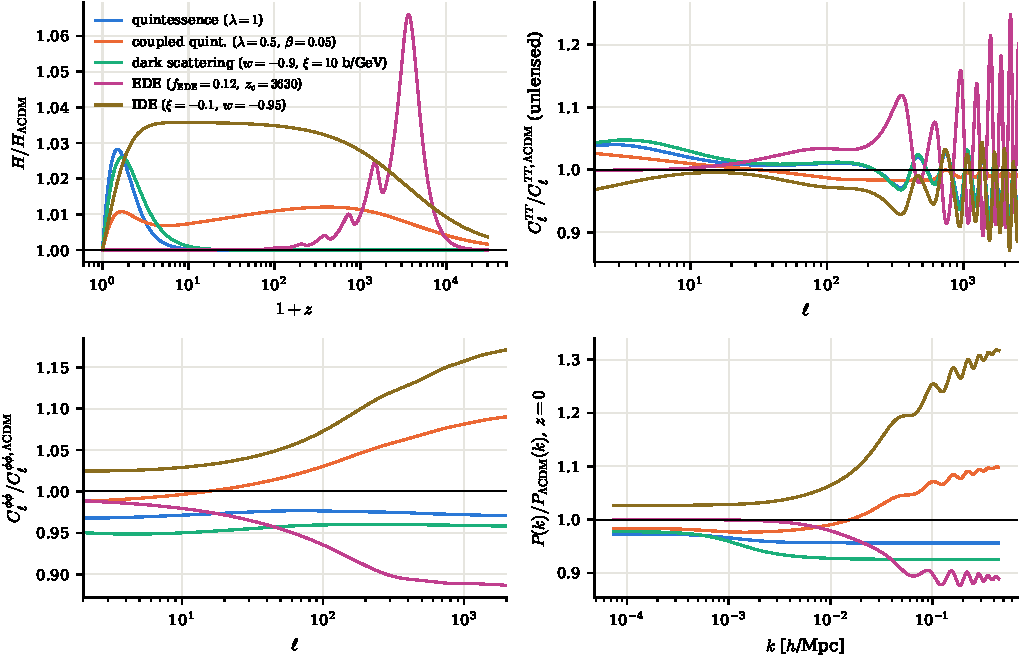
\includegraphics[width=0.85\textwidth]{models_de}
\caption{Dark-energy models and dark-sector interactions relative to $\Lambda$CDM: expansion rate, unlensed TT
spectrum, lensing potential and matter power spectrum today.}
\label{fig:models_de}
\end{figure*}

\begin{figure*}
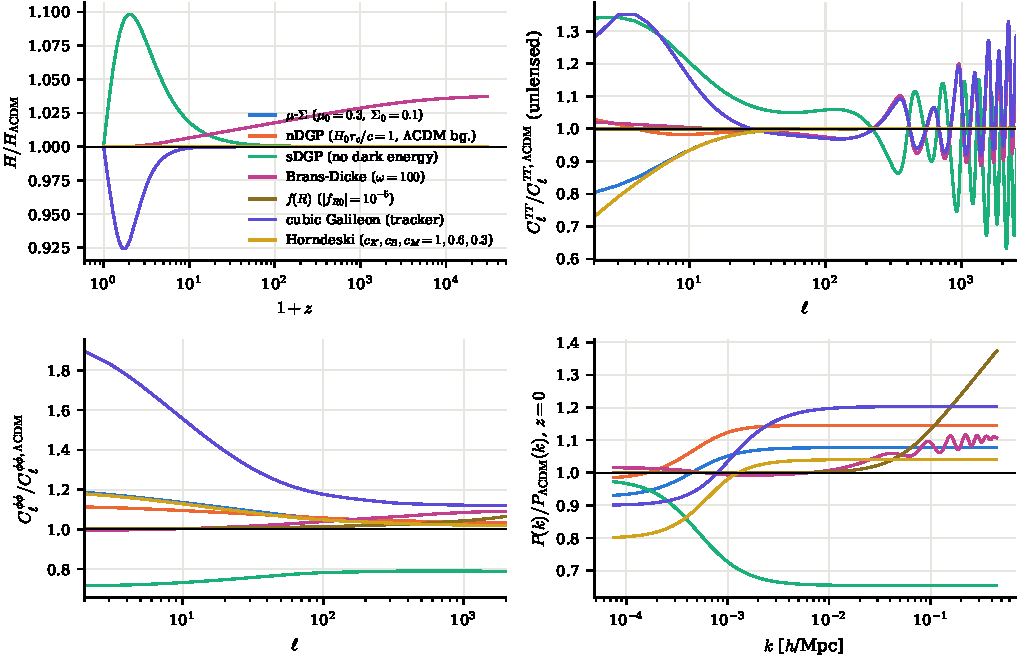
\includegraphics[width=0.85\textwidth]{models_mg}
\caption{Modified-gravity models relative to $\Lambda$CDM, as in Fig.~\ref{fig:models_de}.}
\label{fig:models_mg}
\end{figure*}

\subsection{Discussion}

The models act on the observables in four ways (Figs.~\ref{fig:models_de}--\ref{fig:models_mg},
Table~\ref{tab:models}).
\begin{itemize}
\item \emph{Late-time expansion.} Thawing quintessence raises $H$ at $z\lesssim2$. It slows the growth
      ($\sigma_8$ lower by 2\%) and changes the ISW plateau of TT at $\ell\lesssim20$.
\item \emph{Dark-sector interactions.} These act on the dark matter directly. The fifth force of coupled
      quintessence and the energy outflow of IDE (with $\xi<0$) both enhance the growth of sub-horizon modes, by
      7\% and 25\% in $P(0.1\hMpc)$. IDE also has more
      dark matter in the past, which raises $H$ by about 3\% at high redshift and shifts the acoustic peaks. The drag of
      dark scattering suppresses the growth by 7\% (with $w>-1$).
\item \emph{Modified gravity.} $\mu$--$\Sigma$, nDGP, Brans--Dicke, the Galileon and Horndeski strengthen gravity below
      the horizon. The result is a scale-independent enhancement of $P(k)$ on small scales, between
      4\% (Horndeski) and 20\% (Galileon). $f(R)$ gives
      a scale-dependent enhancement that grows towards the Compton scale. The lensing potential also changes,
      through $\Sigma$ or through the running Planck mass. The self-accelerating DGP branch weakens gravity and
      expands faster, so $P(k)$ is 35\% lower. The scalar--tensor models with dedicated
      field equations also change the large-scale ISW signal of TT strongly: by up to $+35\%$ for the Galileon (at $\ell\approx4$) and
      $-27\%$ for Horndeski (at $\ell=2$).
\item \emph{Early times.} Early dark energy is the only model that acts before recombination. It raises $H$ by up to
      7\% around $z_c$, which reduces the sound horizon. It also slows the growth of the dark matter while the field
      is significant. At fixed $h$ this shifts the acoustic peaks (the ratio to $\Lambda$CDM oscillates by $\pm9\%$), and
      lowers $P(k)$ on small scales by 10\%. In fits to data the smaller sound horizon is
      compensated by a larger $H_0$, which is why the model has been proposed to resolve the Hubble tension.
\end{itemize}
For every model the code computes the unlensed and lensed CMB spectra and the matter power spectrum with the same
pipeline as for $\Lambda$CDM.
